%  Robotics Text  by Jacob Rosen and Blake Hannaford
% (c) 2007  Jacob Rosen and Blake Hannaford
%

\chapter{Motion Planning}

\section{Problem Statement and Learning Objectives}
% Problem Statement and Learning Objectives for Chapter 08
\paragraph{Problem Statement}

Motion planning is the process of finding a collision free path between two configurations of a manipulator, considering the presence of obstacles in the workspace.  

\begin{figure}\centering
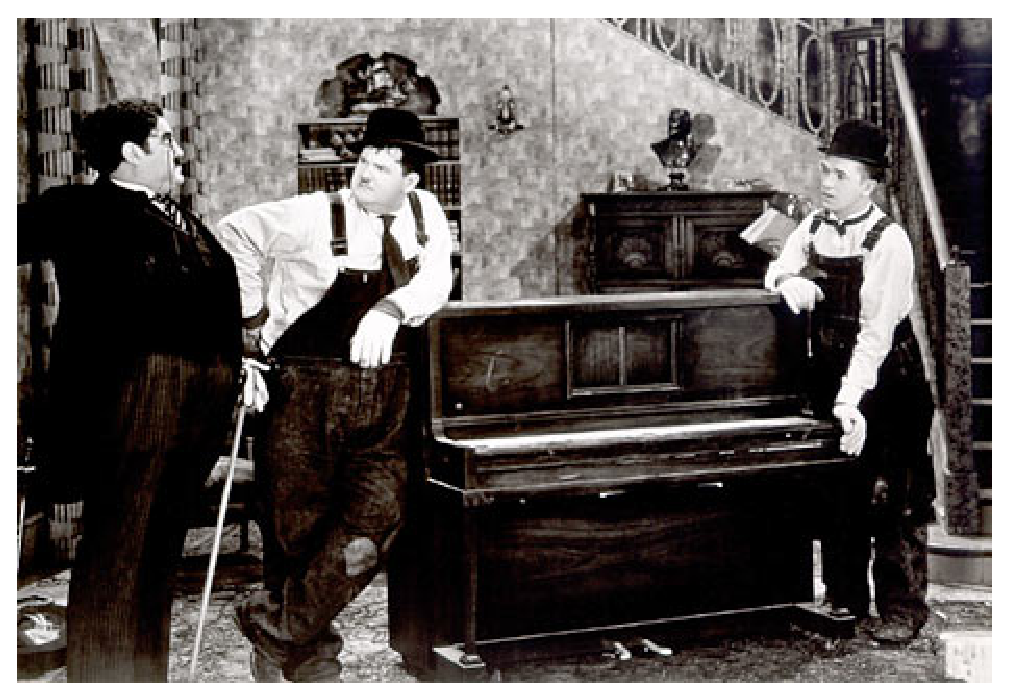
\includegraphics[width=3.5in]{figs08/LaurelHardyPiano.eps}
\caption{How to move the piano up the stairs without touching the walls?}\label{laurelhardy}
\end{figure}

Interestingly, this type of motion planning is usually very easy and natural for humans.  One exception is the case of moving a large bulky object such as a piano through small hallways and doors into a desired room.   This ``piano mover's problem" is similar to the motion planning problem we have posed above.  However if the object (piano) were being manipulated by a (large) serial robot arm, we would also have to consider all potential collisions between the arm and the environment, in addition to the collisions between the piano and the environment. 

\paragraph{Learning Objectives}
Upon completing this Chapter, the reader should be able to
\begin{itemize}
  \item Explain the major problems in motion planning
  \item Identify which ones are most computationally time consuming in typical manipulation applications. 
  \item Explain the Configuration Space.
  \item Describe some sampling based motion planning methods. 
\end{itemize}


\section{Path Planning}
From the standpoint of robot manipulators, the basic problem of motion planning is to find a   path between two configurations of the manipulator (possibly including an object held in the end effector) such that it does not collide with any parts of the environment.  This is a function which humans do so naturally that it might take a moment of reflection to realize why it is a computationally hard problem and why it is still an active area of research.  

First let's consider an extremely simple version of the problem, an obstacle free workspace.   In this case, our path from point $A$ to point $B$ would most likely be a straight line, interpolated in the configuration space (as in Chapter \ref{ChapterTrajectoryGeneration}).  The next problem to take on is to add some obstacles  inside the manipulator workspace.

We must first obtain a representation of the obstacles.   In industrial environments, these are commonly fixtures, racks, conveyors or equipment which are of known dimensions and in fixed locations.   In less structured environments, the obstacles must be sensed, for example by 3D vision systems or laser range finders. 

In either case, we still have the difficult problem of searching for a path of the manipulator through any gaps which exist between the obstacles. 

\section{Configuration Space}

We start by making a clever simplification of the problem originally made by Thomas Lozano Perez.  First, we imagine a world containing a robot arm and a set of static obstacles.  The robot's configuration is represented by a N-dimensional vector such as its joint variables.  \textit{Configuration space} is the space of all possible points representing the robot's joint variables, the same space we have referred to as joint space up until now.   The robot thus becomes a point, and the obstacles become blobs representing all arm configurations in which any part of the arm collides with an obstacle in the end effector space.  The  motion planning task now becomes the apparently simpler one of moving a point from location $A$, to location $B$ between the obstacle blobs.  


\subsection{Collision Detection}

The first problem is to determine whether or not a manipulator in a given pose collides (overlaps in space) with   obstacles in the workspace.   This problem is important because we must find routes through the configuration space in which no collisions occur.  Collision detection algorithms are also central to the related problem of haptic rendering, in which  collisions must be tracked between a user's hand or an object in the user's hand, and a a virtual environment so that force feedback can be computed. 


Note that for practical cases we care about all possible collisions between the arm and the obstacles, not simply those involving the end effector. 

% ** Review of CD algorithms and speedups **

There are many applications for algorithms which can detect if two bodies described by geometrical models are colliding or not.   First, we simplify a few aspects of the problem by making some assumptions:
\begin{itemize}
\item We have a good method for modeling objects such as polygons, implicit surfaces etc. 
\item We model a world containing a number. $N_s$, of static objects, and $N_m$ moving objects.  The static objects model the world around the manipulator, and the moving objects are the links of the manipulator and any object it might be holding. 
\item We assume that the world model, the moving object model, and its position and orientation are modeled exactly.   Although this is unrealistic in most practical applications, we can get around this limitation by artificially growing the objects by an amount equal to the uncertainty in the measurements.
\item We assume a function exists: {\tt check($A$,$B$)} which returns a one if objects $A$ and $B$ intersect.
\item We assume that collisions between the static objects are not interesting. 
\end{itemize}

%Although the {\tt check()} function may be implemented efficiently in some cases, for many realistic models, it is
The {\tt check()} function is not trivial to implement except for basic geometric shapes such as spheres and rectangular solids.  Depending on how detailed the object models are, this function can be computationally expensive. 

Our task is thus to check all the moving objects against all the static objects and against each other.   This would require running the {\tt check()} function $N_m(N_s + (N_m-1)/2)$ times.   For situations where the environment is realistically modeled, this can be computationally prohibitive.   A number of algorithms speed this up by simplifying the search for colliding objects.

One basic speedup uses \textit{axis-aligned bounding boxes} (aabb's, Figure \ref{aabb}).  A bounding box is a rectangular solid  which just encloses an object model.  ``Axis aligned'' means that the boxes are aligned with the $x,y,z$ axes of the Cartesian space.  

\begin{figure}
\centering
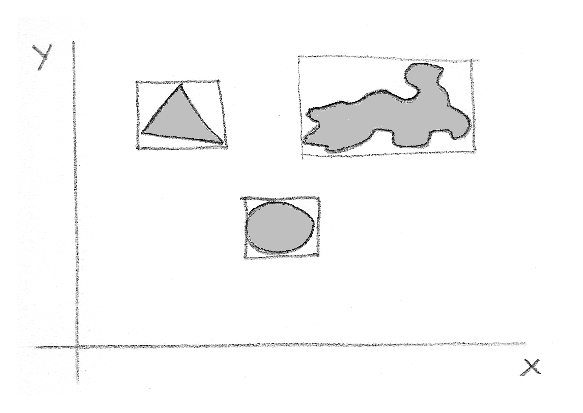
\includegraphics[width=3.5in]{figs08/axisalgnbb.eps}
\caption{Three 2D objects shown with their axis-aligned-bounding-boxes (aabb's).}
\label{aabb}
\end{figure}


Once aabb's are defined for each obstacle, they can be kept in a list.   The lists can be sorted in the $x,y,z$ directions and then rapidly checked for overlaps.   If two bounding boxes overlap in all three axes, then the objects inside must be checked for collisions.    One problem with aabb's is that they must be recomputed for moving objects, especially as their orientation changes.   A second  problem is that they can be unnecessarily large, for example, with a diagonal object, generating too many checking steps (Figure \ref{aabbproblem})
 
\begin{figure}
\centering
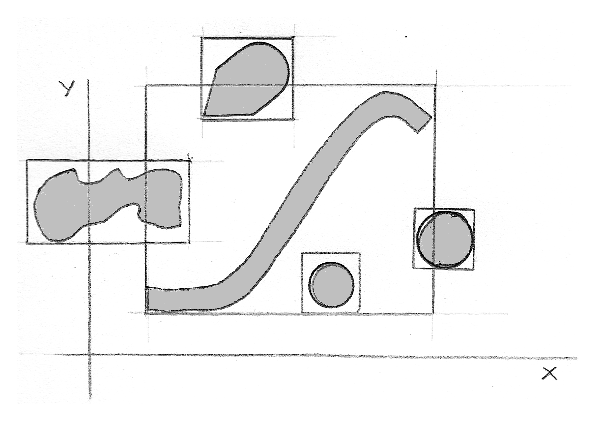
\includegraphics[width=3.5in]{figs08/axisalgnbb2.eps}
\caption{axis-alinged bounding boxes can generate excessive checking when the object is elongated and diagonal. }
\label{aabbproblem}
\end{figure}


An improvement on aabbs are \textit{oriented bounding boxes} (obb's).   In this method, an algorithm computes the smallest rectangular solid of any orientation which can enclose a given object.  Although the algorithm to check obbs for collisions is a bit more involved than checking aabb's, it is still   faster than checking general objects.   Finally, bounding boxes can be arranged hierarchically in a tree so that the number of bounding box checks can be further reduced.

Finally, another class of speedups can be developed by exploiting what is known as temporal and spatial coherency.   In realistic applications, a robot can change its position only a small amount between control samples.   These algorithms exploit this fact by checking for collisions only in an immediate neighborhood of the current position.  When properly implemented this can substantially reduce the computation.

In configuration space, the collision detection task becomes very simple. At each point in the configuration space, the robot is either colliding with an obstacle or it is not.   Each blocking obstacle in the Cartesian space, defines a blob of points in the configuration space.  The set of all such points, due to all obstacles, is called the forbidden region.  The complement of that space is the free region.  At any configuration space  point we can ask ``Does the manipulator point occupy any of the blobs in configuration space?"

\subsection{Computing Obstacles in Configuration Space}

However, the simplification of configuration space generates a new and difficult problem: how to find the c-space blob corresponding to each obstacle in the end effector space.  This is another computationally intensive problem which must be solved prior to motion planning.   Assuming the c-space blobs have been found, we can verify that both the starting and ending configurations are reachable without collisions.   Then the motion planner must find a continuous path through the free region from start point to the goal point.

A naive approach to  the motion planning problem boils down to the following steps:
\begin{enumerate}
 \item Obtain a geometric model of the entire workspace including all obstacles. 
 \item Obtain a collision detection algorithm which can return a single bit for any point, $P$, in configuration space.  If the configuration, $P$, is one in which any part of the robot arm collides  with one or more obstacles, return 1.  If there is no collision, return 0.
 \item Use the collision detection algorithm to obtain a description of the free space. 
 \item Plan a path through the free space to the goal point. 
\end{enumerate}

However, in a realistic problem with multiple obstacles of arbitrary shape, computing the forbidden region (or its complement the free space) is prohibitively difficult.  Thus many realistic motion planning problems must be solved without generating the complete c-space!   For now however we will study a simple planar 2D example so that the free space of the configuration space can be computed.

 Most algorithms which compute explicit representation of the obstacles rely on models such as polygonal models or traingular meshes.   Although  algorithms exist which can compute a c-space boudary representing the collisions of one polygonal solid with another, their complexity grows very rapidly with the c-space and the number and complexity of obstacles so that they are prohibitive for many realistic cases.

\subsection{2-D computational example}
In this section we will illustrate some of these issues with a very simple implementation for a two dimensional example.  It will be obvious that the   algorhithms presented here are rudimentary.  However they are given to illustrate the types of computations which must be scaled up for use with actual manipulators in 3D. 

 We consider the two-link planar manipulator of Example 4.\ref{2LinkJointLimits} (page \pageref{2LinkJointLimits}).  This manipulator had the following parameters:
\[
l_1=4, \qquad l_2=1.5, \qquad 0 \leq \theta_1 \leq 180^\circ \qquad -90^\circ \leq \theta_2 \leq 180^\circ
\]


\begin{figure}\centering
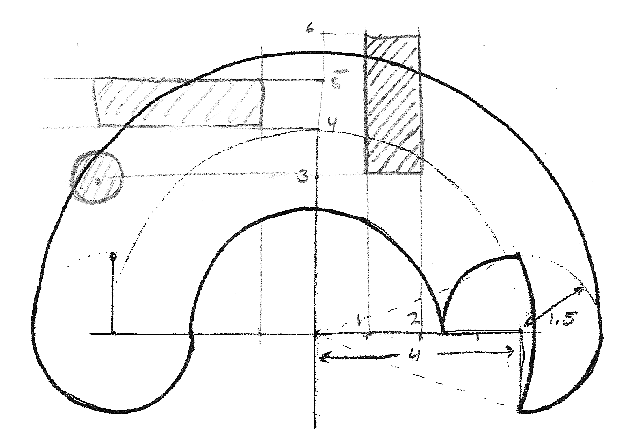
\includegraphics[width=4.0in]{figs08/worksp_obs.eps}
\caption{Workspace from Example 4.\ref{2LinkJointLimits} with the addition of two rectangular and one circular obstacles.}\label{WorkspaceWithObstacles}
\end{figure}

We will add a set of obstacles consisting of rectangles and circles (Figure \ref{WorkspaceWithObstacles}). 
How can we map these obstacles from the workspace to the joint space?  It is very easy to check whether or not a point is inside a circle or a rectangle.   However, we must check for collisions with any point in the arm.   To approximately check this, we will generate a series of points along the arm with a Scilab function {\tt pointcloud(N,t1,t2)} where {\tt N} is the number of points to distribute along the arm, and {\tt t1,t2} are the values for $\theta_1$, and $\theta_2$.  A representation of the arm model used by {\tt pointcloud(10,45,30)} is given in Figure \ref{TwoLinkPointCloud}.   The algorithm takes care to make sure that in addition to N evenly spaced points,  the elbow and the end point are also labeled.

\begin{figure}\centering
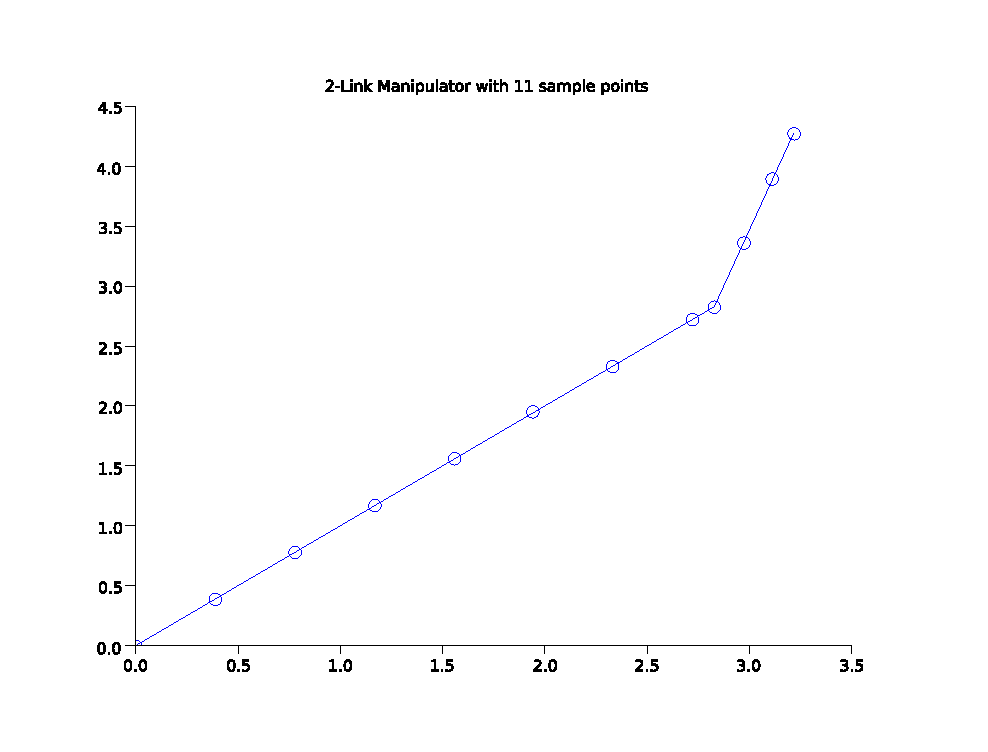
\includegraphics[width=3.5in]{figs08/two_link_pts.eps}
\caption{Basic 2-link manipulator with 11 points distributed along its length.}\label{TwoLinkPointCloud}
\end{figure}

Our second scilab function accepts a series of points generated by {\tt pointcloud()}, and checks them against a rectangle.  It returns a 1 if any point is inside the rectangle.  This function is called {\tt checkrect(v,r)} where {\tt v} is the set of points generated by {\tt pointcloud} and {\tt R} is a vector containing the boundaries of the rectangle, \textit{[xmin,xmax,ymin,ymax]}.  For the first rectangular obstacle (upper right of Figure \ref{WorkspaceWithObstacles}),

\begin{center}
{\tt R = [ 1, 2, 3, 6 ]}
\end{center}

Finally, we make a script {\tt confmap.sci} which loops through joint space.  Each value of $\theta_1,\theta_2$ generates a pose of the manipulator.  At each  pose, the points distributed along the manipulator are checked against the obstacles, and the joint angles are recorded if any of them collide with an obstacle.


\begin{figure}\centering
\begin{tabular}{cc}
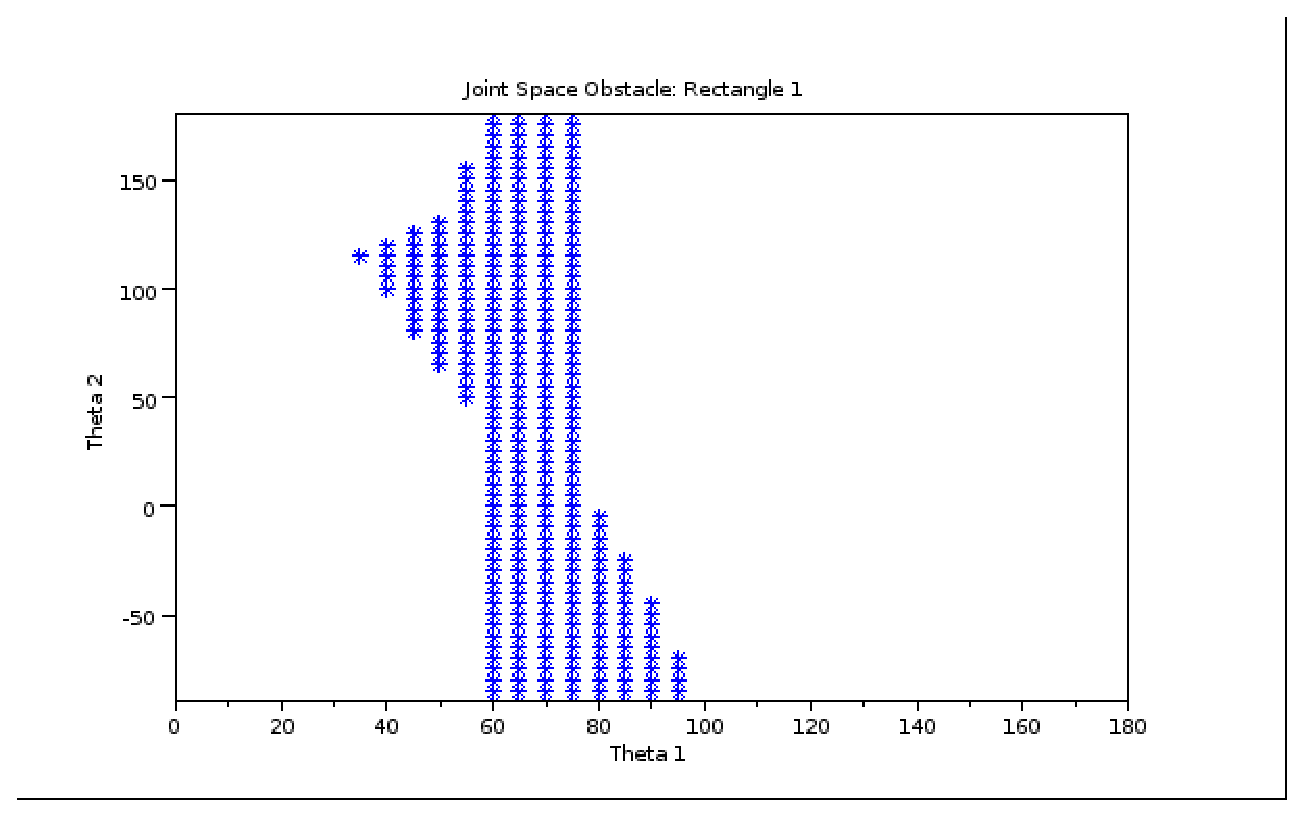
\includegraphics[width=3.0in]{figs08/jobs_rect1.eps} &
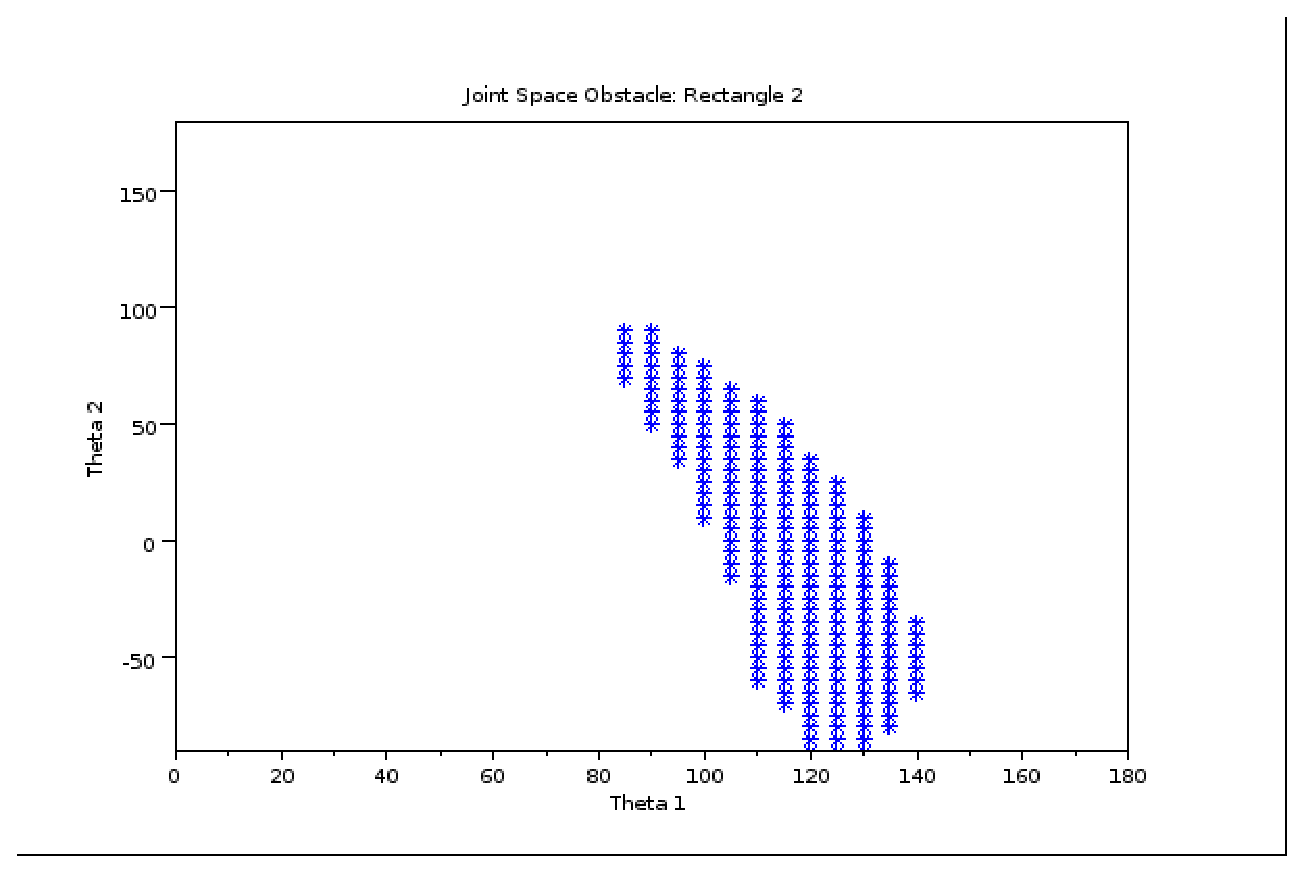
\includegraphics[width=3.0in]{figs08/jobs_rect2.eps} \\
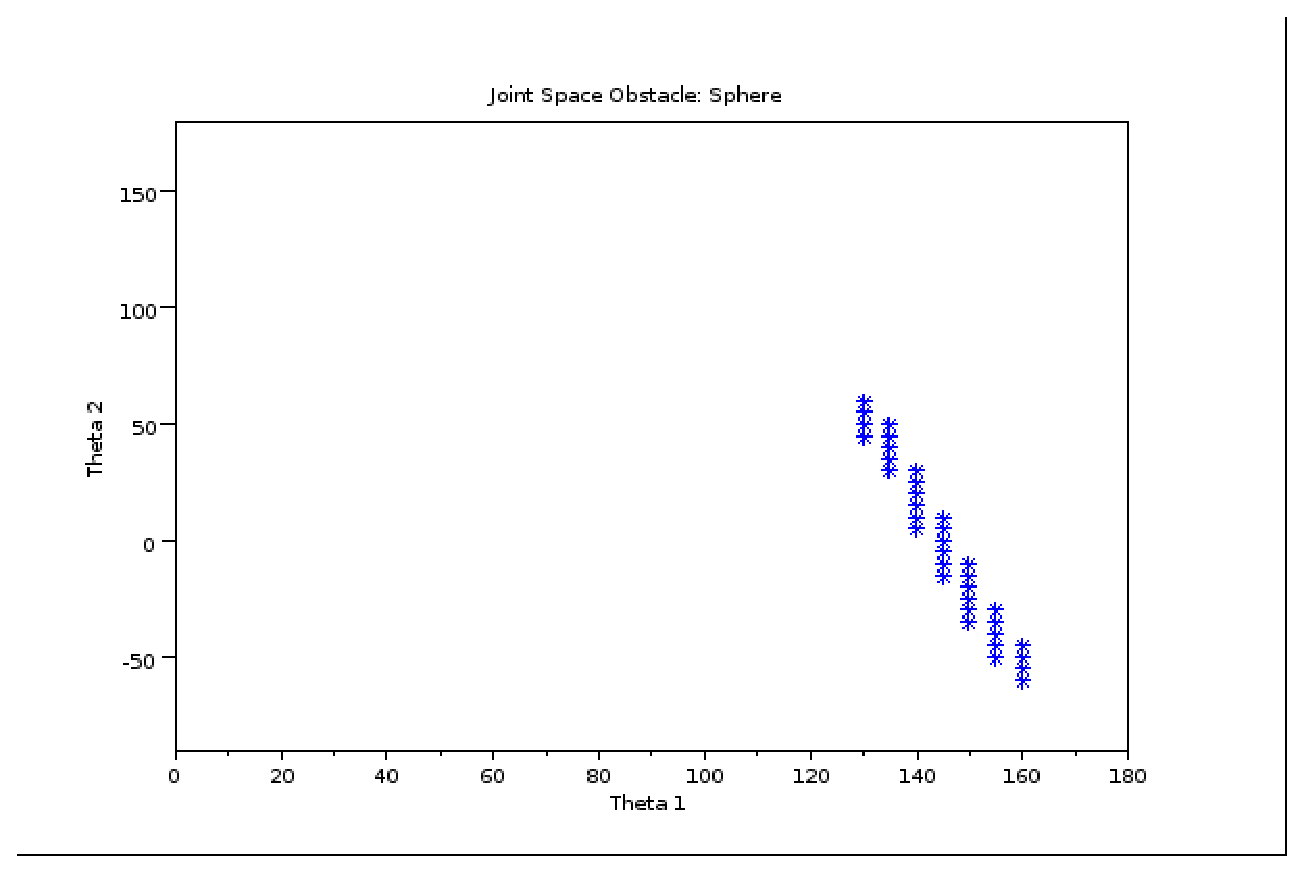
\includegraphics[width=3.0in]{figs08/jobs_sph.eps}   &
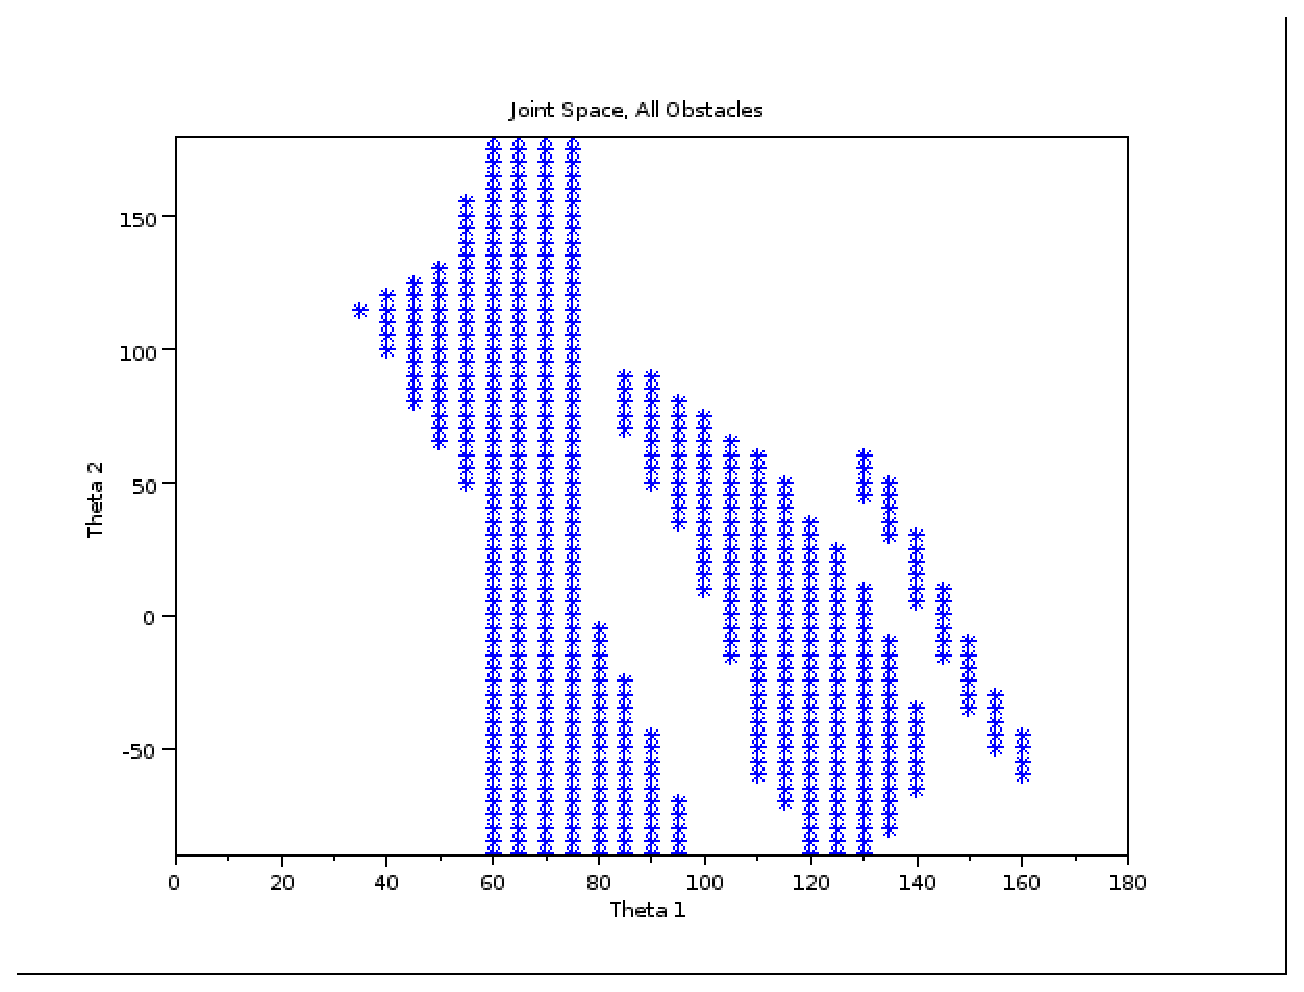
\includegraphics[width=3.0in]{figs08/jobs_all.eps}
\end{tabular}
\caption{Computational results of 2-link planar arm configuration space with up to three obstacles as shown in Figure \ref{WorkspaceWithObstacles}. Configuration space is plotted only within the joint limits.}\label{CspaceObs}
\end{figure}
 

Running {\tt confmap.sci} with rectangle 1, gives the configuration space obstacle shown in Figure \ref{CspaceObs}, upper left.  Our second rectangle (upper left) can be similarly checked ({\tt R2=[-5,-1,4,5]}) to generate the c-space obstacle of Figure \ref{CspaceObs}, upper right. Our circlular obstacle can be checked with a similar function {\tt checksph(v,S)} where {\tt  S = [center\_X, center\_Y, radius]}.  For {\tt S = [-4.2, 3, 0.333]}, we get the configuration space obstacle shown in Figure \ref{CspaceObs}, lower left. Finally, we can consider all obstacles simultaneously and get the set of obstacles shown in Figure \ref{CspaceObs}, lower right.

We can see from Figure \ref{CspaceObs}, lower right, that there can be no path from the free region approximately defined by $\theta_1 < 50^\circ$ and the other region approximately defined by 
$\theta_1 > 80^\circ$ which does not violate the R1-obstacle or the joint limits.   However this fact is not obvious from looking at the workspace and the obstacles (Figure \ref{WorkspaceWithObstacles}).   Rectangle 1 blocks all motion between these two regions because the elbow (always 4 units from the origin) cannot avoid passing through it.


\section{Static Planning for Obstacle Avoidance}

In this section, we assume that the forbidden region of the configuration space is known.   Even so, it is still not trivial to find a pathway through the obstacles.   We need a method to represent the possible pathways 


\begin{figure}
\centering
\includegraphics[width=3.5in]{figs08/voronoi.eps}
\caption{Voronoi diagram for the obstacles of Figure \ref{WorkspaceWithObstacles}.
}\label{Voronoi}
\end{figure}

\subsection{Voronoi Diagrams and Graph Search} \label{VoronoiAndGraph}

An important tool for understanding the free region is the Voronoi diagram.  To construct the Voronoi diagram, we identify all points in the free region which are equidistant between two obtacles.  In 2D space, these points lie along a line.   Such lines merge at points which are equidistant from three or more obstacles which we call nodes.  Once the Voronoi diagram is computed, we have a graph which identifies potential collision free pathways between regions of the c-space.   The Vornoi diagram for the 2D example we have been studying is shown in Figure \ref{Voronoi}.

With a Voronoi diagram in place, the path planning algorithm can be expressed as
\begin{enumerate} 

 \item Find the nearest point on the Voronoi diagram from the start point, and the nearest node to that point. 

 \item Find the nearest point on the Voronoi diagram from the end point, and the nearest node to that point. 

 \item Abstract the Voronoi diagram into a graph.

 \item Search the graph for the shortest (by some measure) pathway between the start and end nodes. 

 \item Create a series of joint space trajectories, following the selected segments on the Voronoi diagram between start and end points. 

\end{enumerate}


\subsubsection{Search}

The Voronoi graph has some important properties. First, (unlike transform graphs of Chapter 2)  it is an undirected graph because there is no inherent direction between the nodes of the Voronoi diagram.   Second, we can compute the length of each edge on the Voronoi graph and use this length as a ``weight" on each edge.  Thus our graph is a undirected, weighted graph. 

Once a graph has been constructed based on the Voronoi diagram, a route must be found by searching through the graph.  There are many published algorithms for searching undirected weighted graphs for the ``best" route from one node to another known as ``graph search" or ``pathfinding" algorithms and many of these have been around since the one developed by famous computer scientist Edsger Dijkstra in the 1950's.   Most of the research on search  algorithms since then is aimed at maximizing the speed or performance of the search as the size of the graph increases. 

Among the attributes of a search algorithm that we care about are
\begin{itemize}
  \item Whether or not it finds the optimum path or just a correct path. 
  \item Whether or not it is guaranteed to find a path if such a path exists.
  \item If heuristics are used to speed up the search, do the heuristics result in sub-optimal paths being returned?
  \item The way its computation cost scales with the problem size (``Big-O" notation).
\end{itemize}

The Voronoi diagram approach converts the planning problem to a graph search problem.

\vspace{0.2in}
\begin{tabular}{|c|c|} \hline
Voronoi Based  Methods & \\ \hline \hline
Advantages		                   &   Disadvantages          			\\ \hline
 Can use robust graph search algorithms.   &   Requires full knownledge of c-space     	\\ \hline
 Deterministic				   &                                            \\ \hline
\end{tabular}


\subsection{Potential Fields}

If the entire configuration space and forbidden region are known, another approach to planning a path has been developed using an analogy to the motion of particles in energetic fields such as electric fields, the ``Potential Field Method".   In this approach, we try to simulate a physical situation where a particle has its maximum energy at the start point, and its minimum energy at the end point.  Obstacles are represented as regions of very high energy and a ``potential field" function on the c-space is created by generating a function combining these two energies.  A virtual particle is placed at the start point and at each time step, the algorithm computes a local gradient of the potential function and the particle is moved by an increment in the direction of steepest descent.  

\begin{figure}
\centering
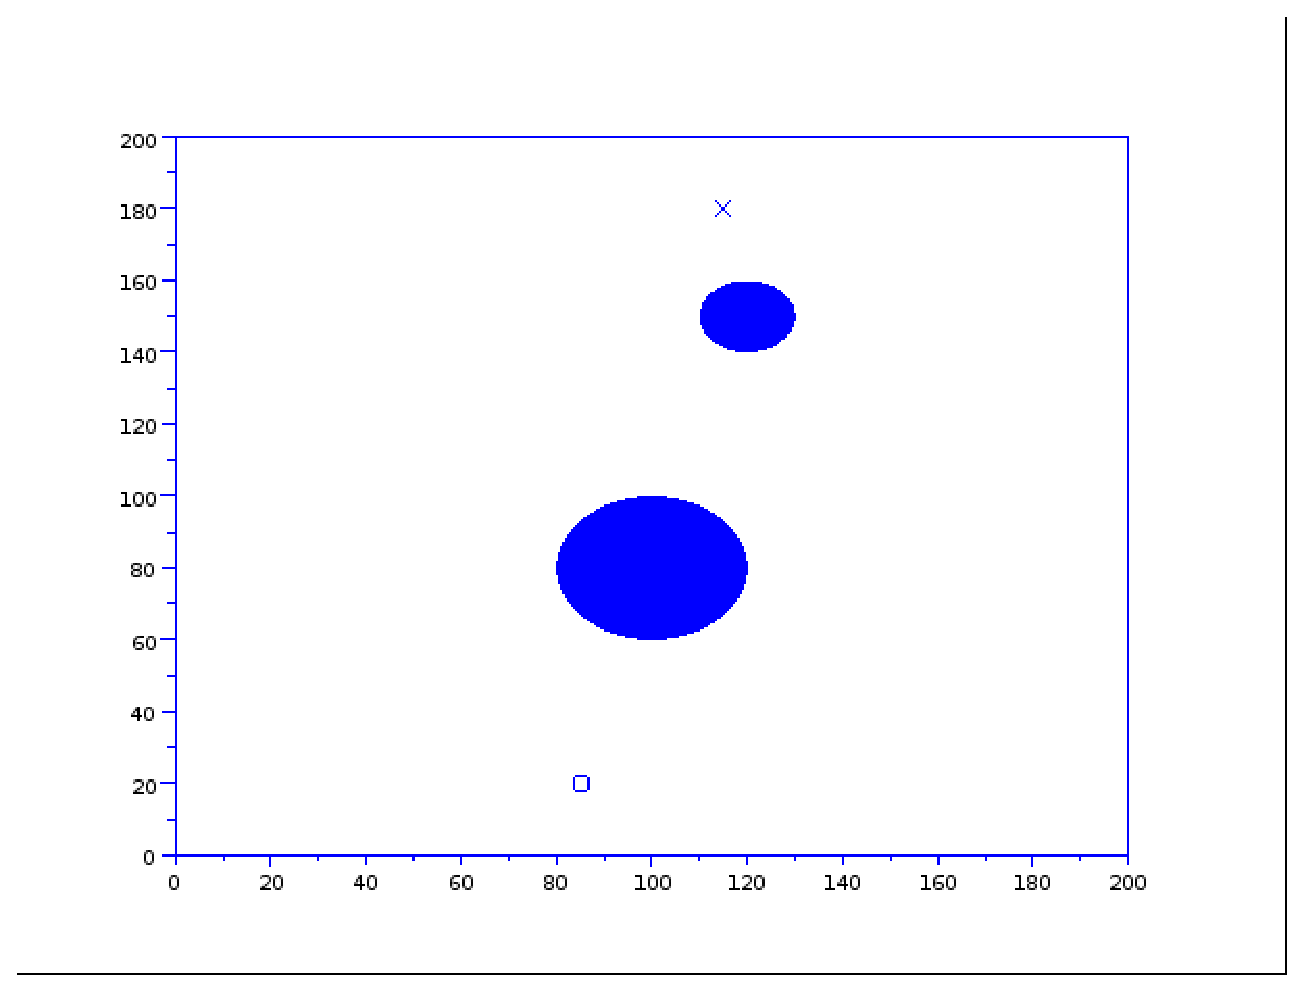
\includegraphics[width=3.5in]{figs08/schem.eps}
\caption{2D configuration space with a start point ('X') a goal point ('O'), and two basic obstacles.
}\label{SchematicConfigurationSpace}
\end{figure}

Consider the 2D configuration space shown in Figure \ref{SchematicConfigurationSpace}.  Assume we have identified a start point ('X'), a goal point ('O'), and that there are two obstacles.  These two obstacles are rather unusual in that they become perfect circles in configuration space!  To construct the potential function, we need two properties.   First, the function must have a minimum at the goal point.   An example of such a function is a basic parabola:
\[
p_g = \left( (x-g_x)^2 + (y-g_y)^2 \right)m
\]
where $m$ is a scaling factor to set the height of the parabola.   Second, the potential function must have high values inside the obstacles.  Ideally, this high ``potential" smoothly descends within the neighborhood of the obstacle.  For circular obstacles, such a function is 
\[
p_o = \left \{ \begin{array}{cc} 1.0 &  r < R \\  
                           1.0 -  3 \frac{r^2}{d^2} - 2\frac{r^3}{d^3} & r \ge R \\
               \end{array}
      \right .
\]
where $r$ is the distance of the current $x,y$ point from the center of the obstacle, $R$ is the radius of the obstacle, and $d$ is the size of the neighborhood of the obstacle.  We can combine these functions using the $max()$ operator.   For a space in which there is just one obstacle:
\[
p(x,y) = max(p_g,p_o)
\]
A 3D plot of such a function for the situation shown in Figure \ref{SchematicConfigurationSpace} is given in Figure \ref{3DplotPotentialFunction}.

\begin{figure}
\centering
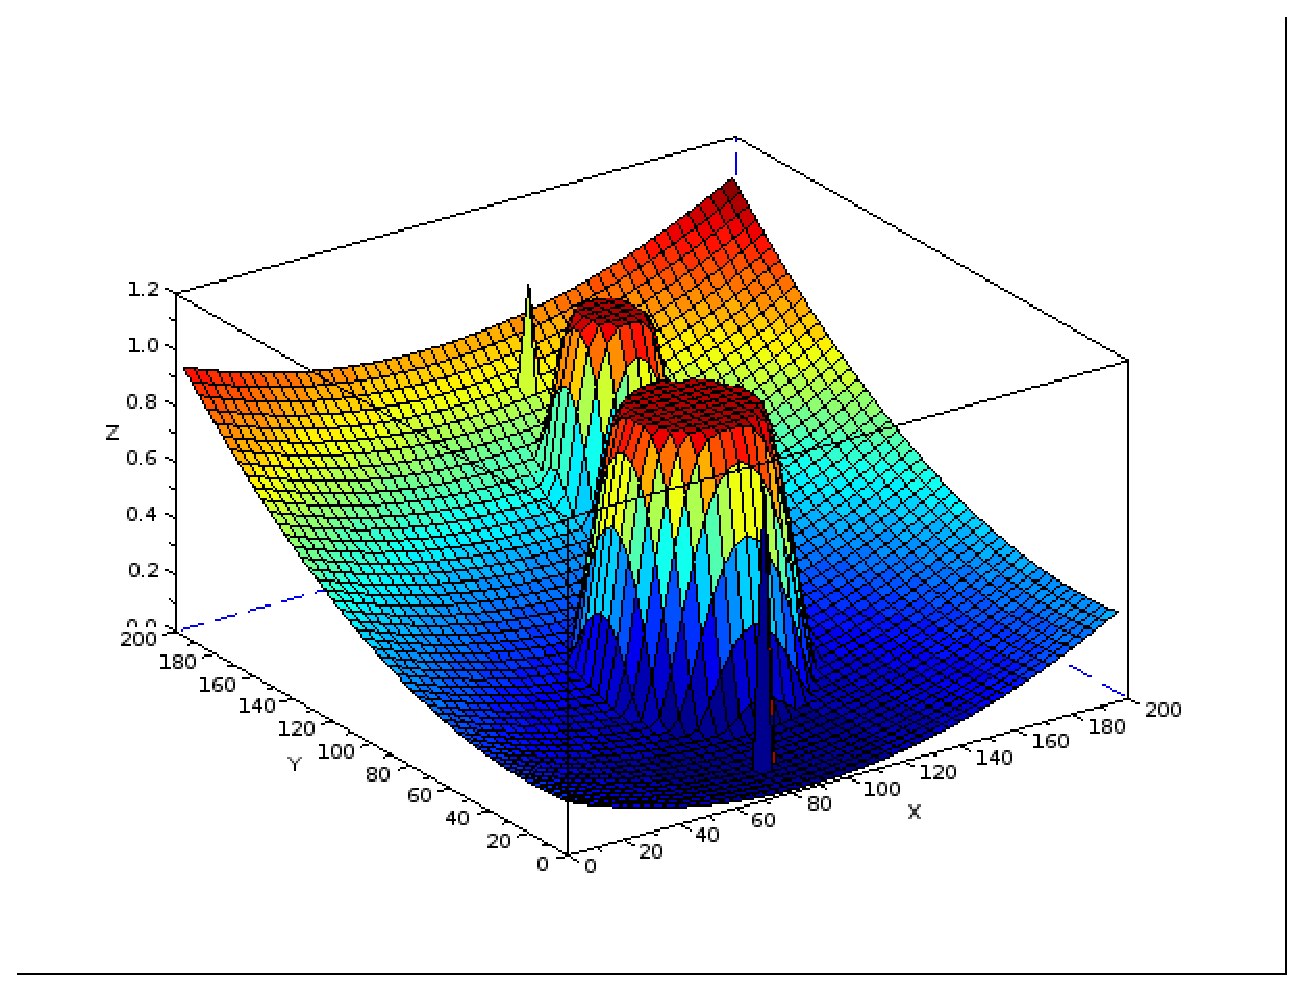
\includegraphics[width=3.5in]{figs08/3d.eps}
\caption{3D plot of the potential function on the 2D configuration space. Start and end points are indicated by spikes.}\label{3DplotPotentialFunction}
\end{figure}

Once the potential function is constructed, we can use a numerical method to estimate the local gradient of the potential function and to move in the negative gradient direction.  We can terminate this process when (if!) we find ourselves in a small neighborhood of the goal point.  A very simple algorithm which approximates this is the following pseudocode:

\begin{verbatim}
i = si;  j = sj;    //  initialize i and j to start point indices
while((i-gi)^2+(j-gj^2) > 2)   // distance to goal
   {
   find smallest value of P(i,j) in all neighboring squares
   i = imin ; j = jmin; 
   }
\end{verbatim}

This algorithm was run on the situation of Figure \ref{SchematicConfigurationSpace}.   The resulting pathway is superimposed on a contour plot of the same potential function as Figure \ref{3DplotPotentialFunction} in Figure \ref{ContourWithPlan}.

\begin{figure}
\centering
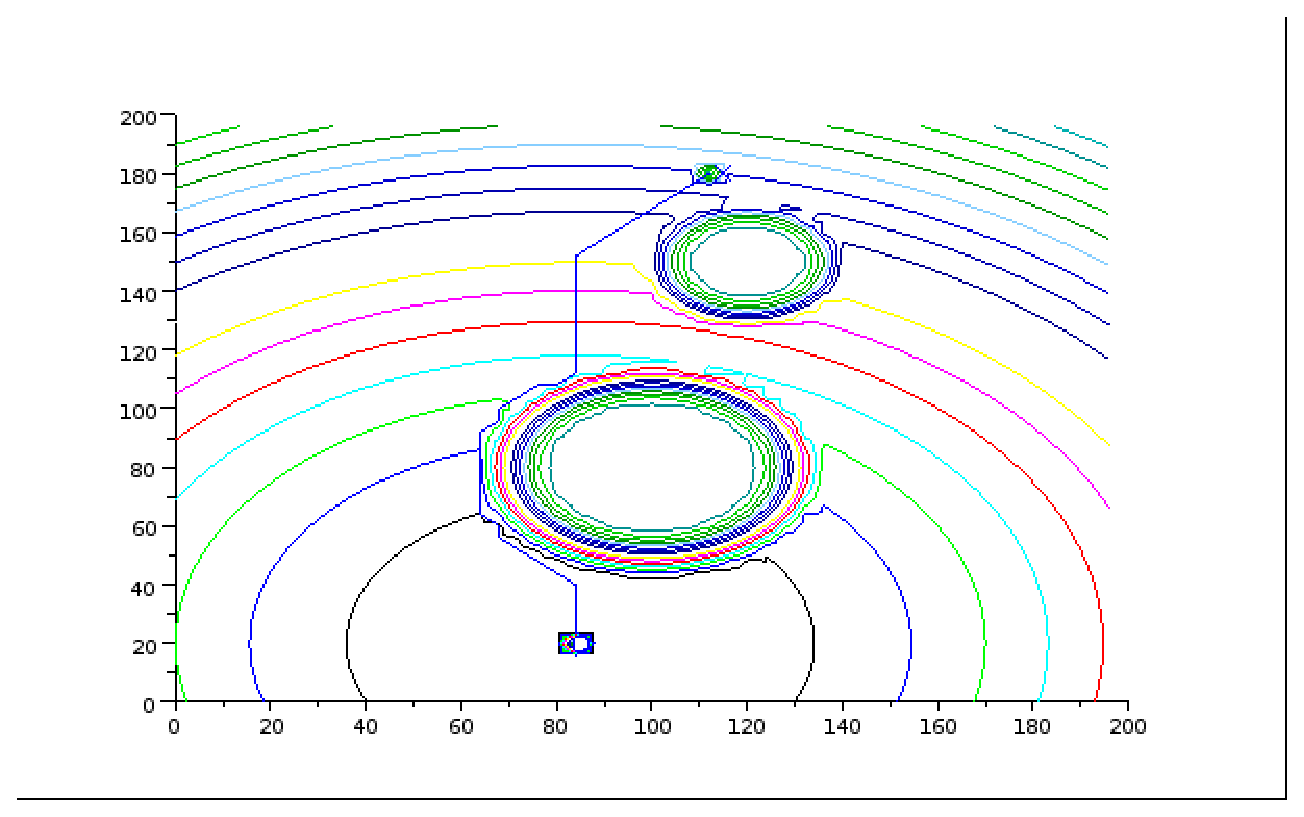
\includegraphics[width=3.5in]{figs08/contourwplan.eps}
\caption{A trajectory from start to goal generated by basic gradient descent algorithm.
}\label{ContourWithPlan}
\end{figure}

The Potential Function approach has converted the planning problem to a gradient descent numerical optimization problem.   

\vspace{0.2in}
\begin{tabular}{|c|c|} \hline
Potential Function Method & \\ \hline \hline
Advantages		    &  Disadvantages          			\\ \hline
Conceptually clear.	    &  Can stick on local minima       		\\ \hline
Well known gradient descent algorithms,   &  Requires full C-space to be computed   	\\ \hline
\end{tabular}
 
\subsection{Sampling Based Methods}

The examples of the previous sections rely on at least one major assumption.  They  assume that the entire configuration space can be computed and represented within reasonable computing resources.  However, there are many aspects of computing and representing the entire configuration space which are very difficult.  The configuration space of a useful manipulator is at least six dimensional.
The collision detection process is computationally intensive for a large number of complex-shaped obstacles, and for manipulator links which are realistically modeled. 
Finally, how do we get the model of the environment in the first place?   In many applications at today's frontier, such as service robots in the home, the environment model must be obtained by sensors such as 3D cameras and laser range-finders.  This technology itself requires extensive computation.  If the environment is changing in any way, or the robot arm is on a mobile base, then the entire C-space must be regenerated in real time.
Many of these factors apply to practical cases in which the  computational complexity of generating the configuration space is intractable. 

A class of algorithms called \textit{sampling based methods}, avoids the need to generate the entire configuration space.
These algorithms still assume that the environment is  known so that collision detection between arm and environmental obstacles can still be performed, but they do not require that the entire configuration space be computed explicitly. 

The sampling strategy of motion planning works as follows:
\begin{enumerate}
  \item  Select a set of sample points throughout the C-space.
  \item  Compute collision detection to determine which of these points are in free space. 
  \item  Search for paths between the sample points which are clear of obstacles.  This will require checking all points in the path between free points. 
  \item  The free space points and the free paths between them create a undirected weighted graph which can be searched as in Section \ref{VoronoiAndGraph}.
\end{enumerate}

A sampling based motion planning strategy in which the sample points are selected randomly by a pseudo-random number generator has been called the \textit{Probabilistic Road Map} method (cites?).  Random sampling is not ideal however because it can leave large holes in the space which are unexplored.  An alternative is  a type of deterministic sequence called a {\it quasi-random number} sequence based on a type of sequence called the Van der Corput sequence.  In one dimension, this sequence is easily obtained by 1) converting the integers to binary numbers, 2) reversing the order of their bits so that the highest order bit becomes the lowest order bit, 3) converting back to an integer.  The Van der Corput sequence, and its multi-dimensional variants, have many properties of random sequences, but can guarantee a certain maximum size of the largest gap between points (Figure \ref{cspacescans}).

\begin{figure}
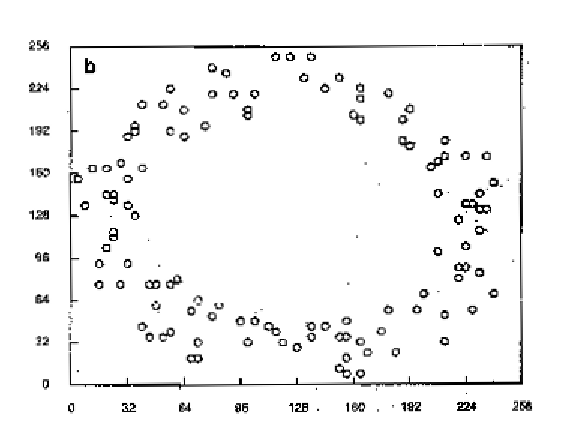
\includegraphics[width=3.25in]{figs08/randomscan.eps}
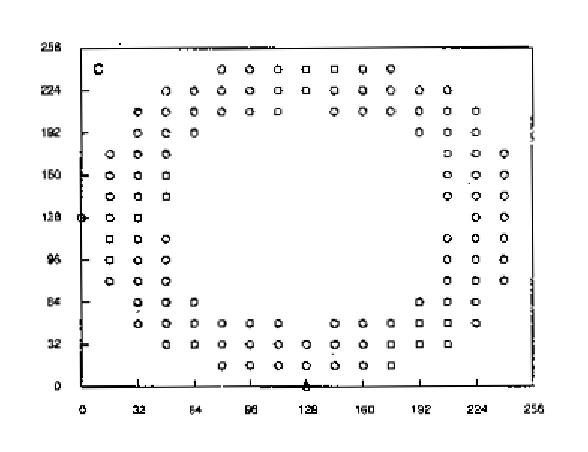
\includegraphics[width=3.25in]{figs08/quasiscan.eps}
\caption{Scans of a donut shaped object performed by a pseudo random number generator (left) and a quasi-random scanning method based on the Van der Corpus Sequence.  Images from B. Hannaford, ``Resolution-First Scanning of Multi-Dimensional Spaces," CVGIP: Graphical Models and Image Processing, vol. 55, pp. 359-369, September 1993.}\label{cspacescans}
\end{figure}

\vspace{0.2in}
\begin{tabular}{|c|c|}
\hline
Sampling Based  Methods & \\ \hline \hline
Advantages		         & Disadvantages          			\\ \hline
Does not require full c-space    &         		\\ \hline
Can use robust graph search algoritms.   &     	\\ \hline
\end{tabular}

\section{Dynamic Constraints}
Dubowsky work. 

\section{Planning With Moving Obstacles ??}
(Fiorini ??)




\section{Summary of Notation}

% Summary of Notation for Chapter  08

